\newpage
\section{Business Intelligence Basics} \label{toc:grundlagenbusinessintelligence}

In diesem Kapitel werden die Grundlagen für das Verständnis von \ac{BI} gelegt. Der Leser soll folglich in der Lage sein, den
\ac{BI} Prozess zu verstehen, um die Erläuterungen in späteren Teilen der Arbeit nachvollziehen zu können. Um dies zu erreichen,
wird in Kapitel \ref{toc:prozess} der \ac{BI} Prozess an sich erklärt. In den folgenden Unterkapiteln wird auf den
strategischen Mehrwert von \ac{BI} eingangen und inwieweit dieser messbar ist. Dies wird für den letzten Teil der Arbeit wichtig,
um zu verstehen, warum sich ein solches Projekt lohnen könnte. Letztendlich wird in Kapitel \ref{toc:einfuehrungsstrategien}
geklärt, welche Voraussetzungen von betrieblicher Seite gegeben sein müssen, damit eine Einführung von BI erfolgreich ist.

Der Begriff \ac{BI} entstand in den 1990er Jahren und wurde erstmals durch Howard Dressner, einem Analysten der Gartner Group,
geprägt.\footcite[Cf.][p. 96]{watson2007current} Vor dieser Zeit gab es bereits Systeme, wie \ac{DSS} und \ac{EIS}, die das
Management dabei unterstützten, Entscheidungen zu treffen.\footcite[Cf.][p. 1]{foley2010business}\footcite[Cf.][p. 19]{niu2009cognition}
Seitdem haben sich diese statischen Systeme zu dynamischen Systemen weiterentwickelt, die unter den Begriff \ac{BI}
fallen.\footcite[Cf.][p. 26]{yeoh2010critical} Für \ac{BI} gibt es viele verschiedene Definitionen, die sich jeweils in Feinheiten
unterscheiden.\footcite[Cf.][p. 114]{muntean2013agile} Eine allgemeine und plakative Definition ist von Eric Foley in seinem Paper
"`What is Business Intelligence?"' gegeben: "`Business intelligence (BI) is a combination of processes, policies, culture, and
technologies for gathering, manipulating, storing, and analyzing data collected from internal and external sources, in order
to communicate information, create knowledge, and inform decision making. BI helps report business performance, uncover new
business opportunities, and make better business decisions regarding competitors, suppliers, customers, financial issues,
strategic issues, products and services."'\footcite[][p. 4]{foley2010business} Es bedeutet, dass \ac{BI} eine Umgebung ist,
in der Daten gesammelt werden, um Wissen und Entscheidungshilfen zu erzeugen. Es bietet einem zudem die Möglichkeit
betriebswirtschaftliche und prozessuale Unzulänglichkeiten aufzudecken und neue Geschäftsfelder zu identifizieren und
zu analysieren. Die Möglichkeit, mit Hilfe von \ac{BI} innerbetriebliche Optimierungen vorzunehmen, ist die zentrale
Eigenschaft, weshalb \ac{BI} für die Prüfung der Hypothesen dieser Arbeit in Betracht gezogen wird.

\subsection{The Business Intelligence Process} \label{toc:prozess}

Um einen \ac{BI} Prozess zu realisieren, braucht es eine Vielzahl von logischen Schritten, die zusammen als Prozess gesehen
werden.\footcite[Cf.][p. 3]{foley2010business} In Abbildung \ref{figure:biprocessoverview} ist der prinzipielle Aufbau eines
\ac{BI} Prozesses skizziert. Dabei sind die ersten Schritte eher technischer Natur. Dies geht während des Prozesses in Schritte
über, die eher durch betriebswirtschaftliche Sichtweisen geprägt sind. Aus Daten wird folglich Wissen
aufgebaut.\footcite[Cf.][p. 13]{kasemsap2016fundamentals}

\begin{figure}[H]
    \caption{The Business Intelligence Process}
    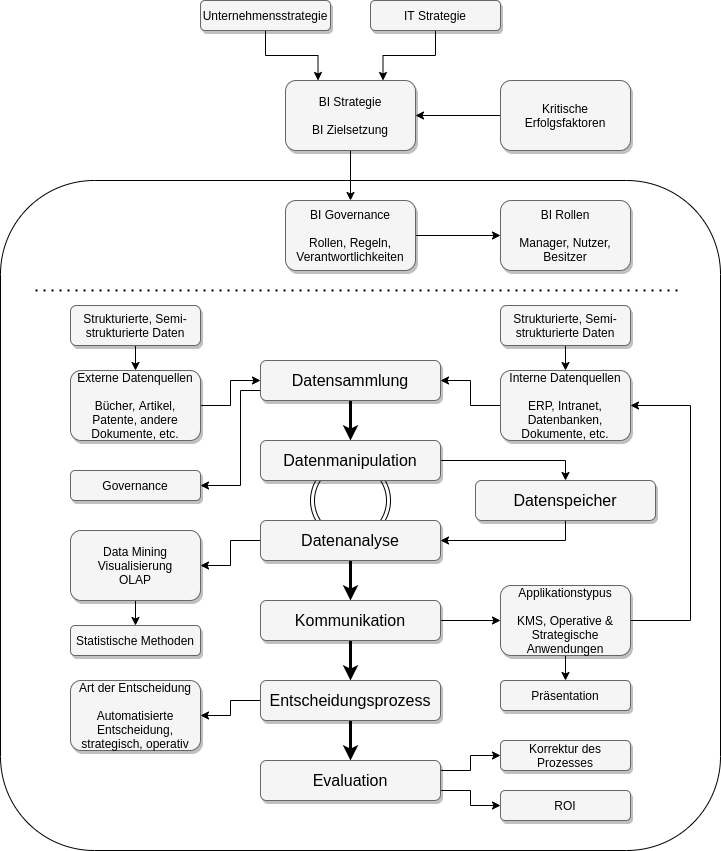
\includegraphics[width=0.7\textwidth]{biprocessoverview}
    \label{figure:biprocessoverview}
    \\
    \cite[Source: Based on][Fig. 2]{foley2010business}
\end{figure}

Ein \ac{BI} Prozess teilt sich in sechs Hauptaktivitäten auf:\footcite[Cf.][Fig. 2]{foley2010business}
\begin{itemize}
    \item \textbf{Datensammlung: }Anfangs werden alle Daten gesammelt. Diesen Schritt benötigt man, um die folgenden
    Prozessabschnitte auszuführen. Dabei können sowohl interne als auch externe Datenquellen verwendet werden. Es muss sich
    dabei nicht zwingend um strukturierte Daten handeln. Es können prinzipiell auch semi- und unstrukturierte Daten
    sein.\footcite[Cf.][p. 465]{ranjan2008business}\footcite[Cf.][p. 3]{hartmann2016capturing}
    \item \textbf{Manipulation der Daten: }In diesem Schritt werden die gesammelten Daten in einer Weise strukturiert, dass
    diese in einem \ac{DW} abgespeichert werden können.\footcite[Cf.][p. 463]{ranjan2008business} Dabei ist das Ziel, eine
    möglichst effiziente Datenbearbeitung zu haben, die auf die Bedürfnisse der Stakeholder und der Nutzer dieser Daten Rücksicht
    nimmt. Am Ende dieses Schrittes werden die Daten in einem "`Data Storage"' (Cf. Fig. \ref{figure:biprocessoverview}) abgelegt.
    Dies ist entweder ein Data Warehouse oder ein Data Mart. Die ersten beiden Schritte des \ac{BI} Prozesses sind daher nichts
    anderes als eine \ac{ETL} Pipeline in welcher die Daten abgefragt, strukturiert und in einem \ac{DW} abgelegt
    werden.\footcite[Cf.][p. 466]{ranjan2008business} Ein solches System kann beispielsweise durch "`Apache Hadoop"' und
    "`Spark"' realisiert werden.\footcite[Cf.][p. 65]{rahman2015big}
    \item \textbf{Analyse der Daten: }Folgend werden die Daten analysiert, die in einem Data Warehouse oder einem vergleichbaren
    System zu finden sind.\footcite[Cf.][p. 16]{kasemsap2016fundamentals} Dies kann durch verschiedenste Systeme erreicht werden
    und ist sehr auf die Zielsetzung des Prozesses zugeschnitten.\footcite[Cf.][p. 21]{niu2009cognition} Deshalb ist es wichtig,
    dass die Anforderungen der Stakeholder akkurat umgesetzt sind, sodass keine falschen Analysen und Ergebnisse präsentiert
    werden und im schlimmsten Fall zu komplett falschen Entscheidungen führen. Bei diesem Schritt kommen unter anderem \ac{OLAP}
    Systeme zum Einsatz, mit denen multidimensionale Vergleiche und Analysen der Daten möglich
    sind.\footcite[Cf.][p. 107ff]{hovcevar2010assessing} Es werden auch weitere Systeme aus den Bereichen maschinelles Lernen
    und Data Mining verwendet.\footcite[Cf.][p. 11]{foley2010business}\footcite[Cf.][p. 80]{yeoh2008managing} Zusätzlich ist
    der Betrieb von Simulationen (beispielsweise Monte-Carlo Simulationen) in diesem Schritt möglich. Letztendlich wird am
    Schluss dieses Schrittes als Ergebnis der Analysen und Berechnungen dem Management Wissen geboten, das gerade in Hinsicht
    auf Entscheidungsprozesse einen Vorteil gegenüber Konkurrenten bietet.\footcite[Cf.][p. 94]{hovcevar2010assessing}
    \item \textbf{Kommunikation und Zugang: }Durch den Schritt der Datenanalyse ist erreicht worden, dass aus Daten Wissen
    extrahiert wurde. Dieses Wissen zugänglich zu machen, ist Aufgabe dieses Schrittes. Hierbei geht es darum, dass das Wissen
    den richtigen Stakeholdern über das richtige Medium zugänglich gemacht wird.\footcite[Cf.][p. 11]{foley2010business} Diese
    Medien können Dashboards, Reporte, Scorecards und andere Methodiken sein.\footcite[Cf.][p. 21ff]{niu2009cognition} Am Ende
    dieses Schrittes ist das Wissen den Stakeholdern zugänglich, sodass mit dem nächsten Schritt begonnen werden kann.
    \item \textbf{Entscheidungsprozess: }In diesem Schritt wird von dem betreffenden Stakeholder die eigentliche Entscheidung
    getroffen.\footcite[Cf.][p. 12]{foley2010business} Dabei werden die aufbereiteten Daten als Unterstützung der Person zur
    Verfügung gestellt. Dadurch kann sie ihre Entscheidungen transparent auf die erhobenen Daten
    stützen.\footcite[Cf.][p. 13]{kasemsap2016fundamentals}
    \item \textbf{Evaluation: }Letztendlich wird evaluiert, ob das \ac{BI} System die erhofften Verbesserungen bzw. Vorteile
    bringt. Dazu kann zum einen gezeigt werden, dass sich das System finanziell lohnt und zum Erfolg des Unternehmens
    beiträgt.\footcite[Cf.][p. 12]{foley2010business} Auf der anderen Seite können in diesem Schritt auch korrigierende
    Maßnahmen eingeführt werden, falls der \ac{BI} Prozess nicht den gewünschten Erfolg brachte.\footcite[Cf.][p. 12]{foley2010business}
    Durch diesen Ansatz gewinnt der gesamte \ac{BI} Prozess einen agilen und zyklischen Charakter.
\end{itemize}

Wie in Abbildung \ref{figure:biprocessoverview} ersichtlich ist, gibt es weitere Faktoren, die zu einem funktionierenden
\ac{BI} Prozess beitragen. Dazu gehört in erster Linie die Strategie und Zieldefinition eines BI Projekts. Diese sind maßgeblich
durch die \ac{CSF} beeinflusst. In Kapitel \ref{toc:einfuehrungsstrategien} werden die Faktoren genauer analysiert, da sie
einen maßgeblichen Einfluss auf eine erfolgreiche Einführung haben. Darüber hinaus gibt es den Punkt der "`IT Governance"'.
Im Falle von \ac{BI} ist damit die Menge aller Richtlinien und der Stellen gemeint, die dafür verantwortlich sind, dass die
einzelnen Bereiche des Projekts klar geregelt sind.\footcite[Cf.][p. 8]{foley2010business} Schlussendlich soll mit
der Einführung dieser Governance der \ac{ROI} des \ac{BI} Projekts gesichert werden.\footcite[Cf.][p. 8]{foley2010business}

\subsection{Added value for businesses} \label{toc:strategischermehrwert}

Bei IT-Projekten ist es meist schwierig, den gesamten Mehrwert für ein Unternehmen abschätzen zu können, der sich primär durch
den \ac{ROI} definieren lässt.\footcite[Cf.][p. 97]{hovcevar2010assessing} Dies liegt an der Aufteilung des Mehrwerts
in finanzielle Faktoren, die vergleichsweise einfach zu benennen sind, und in nicht-finanzielle Faktoren, die indirekt messbar
sind und daher nur schätzbar sind.\footcite[Cf.][p. 93]{hovcevar2010assessing} Dies trifft für \ac{BI} Prozesse zu. Da ein \ac{BI}
Prozess seinen zentralen Vorteil in der Entscheidungsunterstützung des Managements hat und diese sehr komplex sein kann, kann der
finanzielle Einfluss unter Umständen nur abgeschätzt werden.\footcite[Cf.][p. 94f]{hovcevar2010assessing} In Abbildung
\ref{figure:mehrwertbi} sind Mehrwerte gelistet, die ein \ac{BI} Prozess für ein Unternehmen haben kann. Diese sind absteigend
nach der Schwierigkeit der Messung des finanziellen Mehrwerts sortiert.

\begin{figure}[H]
    \caption{Added value of Business Intelligence}
    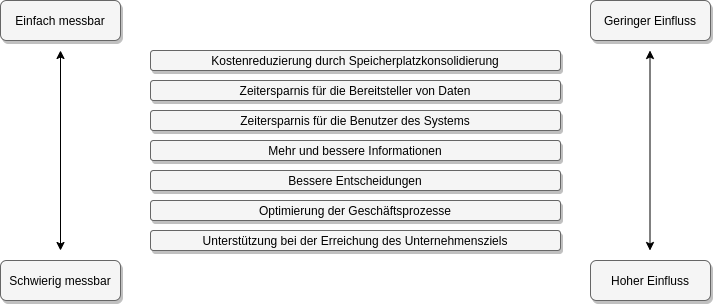
\includegraphics[width=0.85\textwidth]{mehrwertbi}
    \label{figure:mehrwertbi}
    \\
    \cite[Source: Based on][Fig. 2]{watson2007current}
\end{figure}

Nach Abbildung \ref{figure:mehrwertbi} lässt sich der Mehrwert eines BI Prozesses in die folgenden Bereiche
aufteilen:\footcite[Cf.][Fig. 2]{watson2007current}

\begin{itemize}
    \item Durch die Einführung eines Data Warehouses oder eines Data Marts werden unternehmensrelevante Daten für die Analyse
    an einem Ort gespeichert. Es können Kosten für eine Vielzahl heterogener Speicherorte reduziert werden. Die Verfügbarkeit
    der Daten wird verbessert. Dadurch ist eine Kostenreduktion durch ein einheitliches System der Datenspeicherung
    möglich.\footcite[Cf.][p. 105]{azma2012business}
    \item Durch die automatisierte Datenbeschaffung für das Data Warehouse und die schnelle Verfügbarkeit durch \ac{OLAP} Systeme
    ist auch eine Zeitersparnis im Prozess der Datenbeschaffung und -bereitstellung zu messen.\footcite[Cf.][p. 51]{horakova2013business}
    Diese kann in eine finanzielle Größe überführt werden und bei der Analyse des Mehrwerts in Betracht gezogen werden.
    \item Da unternehmensrelevante Daten an einem Ort gespeichert sind und dadurch schnell für die Nutzer verfügbar sind,
    ist eine Zeitersparnis bei den Stakeholdern des Systems messbar.\footcite[Cf.][p. 97]{williams2003business} Wie bei dem
    letzten Punkt kann diese auch der Analyse des Mehrwerts hinzugefügt werden.
    \item Als eines der Ergebnisse des BI Prozesses sind Informationen und Wissen schneller verfügbar. Die Qualität der
    Informationen ist höher als davor, da die Informationen auf größeren Datenmengen, mehr Datenquellen und besseren Analysen
    beruhen.\footcite[Cf.][p. 51]{horakova2013business} Parameter, wie beispielsweise die Informationsqualität sind Faktoren,
    die nur durch Abschätzungen in eine finanzielle Analyse Einzug halten können.\footcite[Cf.][p. 51]{horakova2013business}
    \item Als Konsequenz aus der besseren Informationslage ist nun das Management in der Lage, Entscheidungen besser fällen
    zu können. Wie eingangs beschrieben, kann eine solche Entscheidung aufgrund der hohen Komplexität und der großen Auswirkung
    schlecht finanziell bemessen werden.\footcite[Cf.][p. 51]{horakova2013business} Zusätzlich sind die Opportunitätskosten
    schlecht messbar.\footcite[Cf.][p. 99]{hovcevar2010assessing}
    \item Geschäftsprozesse können mit Hilfe von \ac{BI} optimiert werden. Dies ist aufgrund der besseren Informationslage und
    damit der Möglichkeit, Unzulänglichkeiten zu identifizieren, möglich. Der dadurch erhaltene Vorteil ist ein schwer
    abschätzbarer Punkt, da im Vorhinein nicht absehbar ist, inwieweit Prozessoptimierungen nötig sind und wie sich diese
    finanziell auswirken.\footcite[Cf.][p. 2]{williams2003business}
    \item Eine der Grundlagen für die Einführung von \ac{BI} ist ein klares Unternehmensziel (vgl. Kapitel \ref{toc:einfuehrungsstrategien}).
    \ac{BI} kann helfen dieses schneller und besser zu erreichen. Da aber sehr viel mehr Faktoren als nur ein BI Prozess
    zur Erreichung des Unternehmensziels beitragen, ist es schwierig, den rechtmäßigen Anteil zu identifizieren und in die
    Analyse des Mehrwerts einfließen zu lassen.\footcite[Cf.][p. 51]{horakova2013business}
\end{itemize}

Im Gegensatz zu dem Mehrwert sind die Kosten für ein \ac{BI} Projekt recht einfach abschätzbar, indem diese für die Infrastruktur,
Software und das Projektteam in Betracht gezogen werden.\footcite[Cf.][p. 98]{hovcevar2010assessing} Die Kostenersparnisse
und Einnahmen durch einen \ac{BI} Prozess müssen die Ausgaben übersteigen, damit ein \ac{ROI} messbar
wird.\footcite[Cf.][p. 8]{williams2003business} Nur falls dies möglich ist, kann ein unternehmensweiter Mehrwert des Projekts
identifiziert werden und dadurch auch die Sinnhaftigkeit gegenüber dem Management dargelegt werden. Zusammenfassend ist
feststellbar, dass sich der hauptsächliche Mehrwert von BI folgendermaßen definieren lässt: "`the business value of BI lies in
its effective use within management processes and/or operational processes that drive revenue or reduce
costs."'\footcite[][p. 7]{williams2003business}

\subsection{Voraussetzungen für eine erfolgreiche Einführung} \label{toc:einfuehrungsstrategien}

Die Voraussetzungen, die für eine erfolgreiche Einführung nötig sind, werden in den kritischen Erfolgsfaktoren beschrieben.

\begin{figure}[H]
    \caption{Prerequisites for a successful BI implementation}
    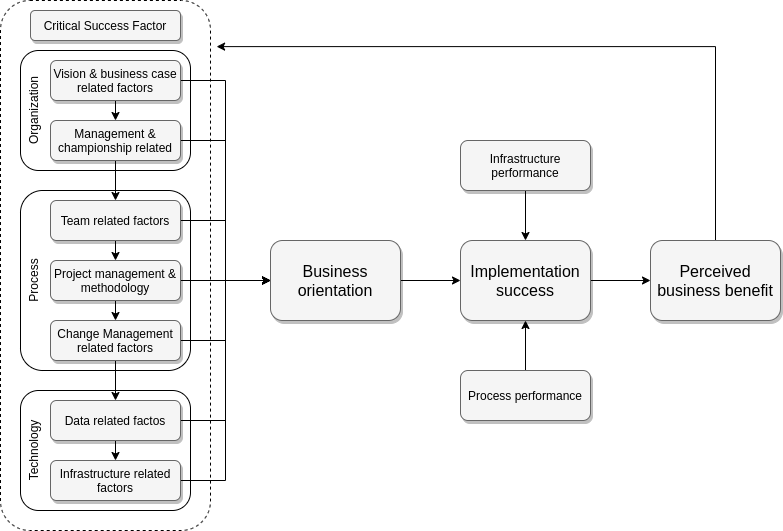
\includegraphics[width=0.85\textwidth]{bisuccessfactors}
    \label{figure:bisuccessfactors}
    \\
    \cite[Source: Based on][Fig. 1]{yeoh2010critical}
\end{figure}

In Abbildung \ref{figure:bisuccessfactors} werden diese Erfolgsfaktoren in drei verschiedene Dimensionen und somit verschiedene
Sichtweisen aufgeteilt.\footcite[Cf.][p. 26ff]{yeoh2010critical} Anhand dieser Dimensionen ist es später möglich, eine
Stakeholderanalyse für einen \ac{BI} Prozess durchzuführen. Die drei verschiedenen Sichtweisen lassen sich wie folgt definieren:

\begin{itemize}
    \item \textbf{Organisationelle Sicht: }In dieser Dimension wird eine Sichtweise aus Richtung der Organisation zu Grunde gelegt.
    Dabei gibt es zwei Punkte, die den Erfolg eines \ac{BI} Prozesses möglich machen. Der erste Punkt verlangt, dass das Projekt
    klare Unterstützung durch das Management erhält. Damit kann sichergestellt werden, dass das Projekt eine genügende finanzielle
    und personelle Ausstattung erhält.\footcite[Cf.][p. 98]{watson2007current} Ein Projektsponsor seitens des Managements ist
    zu empfehlen.\footcite[Cf.][p. 87f]{yeoh2008managing} Der zweite Punkt ist, dass das Projekt eine klare Zielsetzung und Vision
    haben muss.\footcite[Cf.][p. 50]{villamarin2017key} Dies verlangt von einem Unternehmen, welches einen solchen Prozess einführen
    will, eine klare Vision. Anhand dessen ist es möglich, die Projektvision zu formulieren und letztendlich eine klare
    Zielsetzung für das Projekt zu definieren.\footcite[Cf.][p. 87f]{yeoh2008managing}
    \item \textbf{Prozessuale Sicht: }Diese Sichtweise betrachtet die eigentlichen Prozesse und Voraussetzungen auf Projektebene.
    An erster Stelle steht ein Projektmanagement, das in der Lage ist, das Projekt zu leiten. Solch ein Projektmanager sollte die
    technische, organisatorische und prozessuale Sichtweise verstehen.\footcite[Cf.][p. 27]{yeoh2010critical} Er muss mit den
    Prozessen in dem Unternehmen genauso vertraut sein, wie mit den Eigenschaften der technischen Systeme, die zur Lösung der
    Problemstellung verwendet werden.\footcite[Cf.][p. 88f]{yeoh2008managing} Zusätzlich ist eine ausgewogene Teamzusammensetzung
    sehr wichtig.\footcite[Cf.][p. 87f]{yeoh2008managing} Da die Einführung von BI Prozessen typischerweise von
    interdisziplinärem Charakter ist, sollte das Team sowohl aus Spezialisten in der Technik als auch Spezialisten für
    Datenanalyse, Datenpräsentation und Geschäftsprozessen bestehen.\footcite[Cf.][Fig. 7]{muntean2013agile} Zu guter Letzt
    wird eine flexible und agile Entwicklungsweise empfohlen, da gerade \ac{BI} Systeme schnell auf sich ändernde Anforderungen
    reagieren sollen. Nur durch diese Flexibilität ist es möglich schnell zu reagieren, falls etwas geändert, verbessert
    oder aktualisiert werden soll. Eine Methodik, um dies zu erreichen, ist
    Scrum.\footcite[Cf.][p. 164]{isik2011business}\footcite[Cf.][p. 3817]{knabke2013understanding}
    \item \textbf{Technologische Sicht: }Schlussendlich ist die technologische Sichtweise von Bedeutung. Diese teilt sich in zwei
    Themenfelder auf: Auf der einen Seite sind dort die Erfolgsfaktoren, die den Umgang mit den Daten
    betreffen.\footcite[Cf.][Fig. 1]{yeoh2010critical} Diese Faktoren beschreiben primär die Beschaffenheit der verwendeten
    Daten. Dabei werden zwei Anforderungen an die Daten gestellt: Die Daten sollen sowohl eine hohe Qualität als auch eine
    hohe Integrität aufweisen.\footcite[Cf.][p. 163]{isik2011business} Beides könnte zu verfälschten Ergebnissen führen,
    wodurch ein BI System unbrauchbar werden kann. Auf der anderen Seite gibt es Faktoren, die die infrastrukturelle Seite
    betreffen.\footcite[Cf.][Fig. 1]{yeoh2010critical} Die unterliegende Infrastruktur sollte vor allem flexibel und
    skalierbar sein. Diese muss in der Lage sein, auf wechselnde Anforderungen an das Projekt zu
    reagieren.\footcite[Cf.][p. 89f]{yeoh2008managing}
\end{itemize}

Anhand dieser kritischen Erfolgsfaktoren ist es möglich, während der Projektplanung zu überprüfen, ob die wichtigsten
Voraussetzungen für eine Projektdurchführung gegeben sind. Später in dieser Arbeit wird eine solche Analyse konkret durchgeführt.
